\indent\indent Using the \textit{Mask Markers} feature will allow you to manually select badly correlated data in order to hide it from you analysis. Select the markers that do not behave as expected and apply the mask to enhance the analysis results.\\

\begin{figure}[!h]
   \centering
   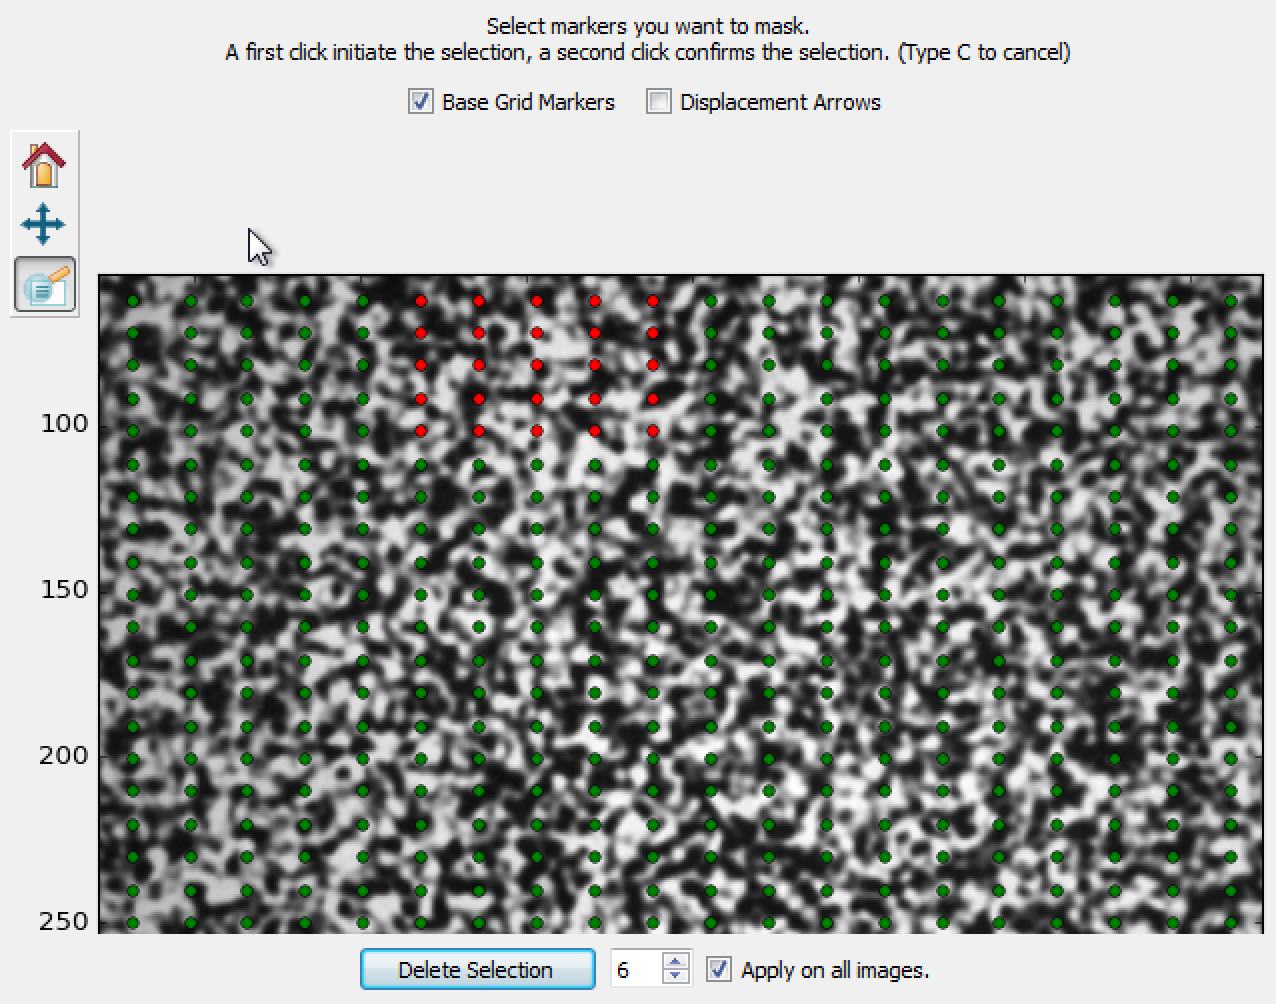
\includegraphics[scale=.4]{mask_markers}
   \caption{Mask Markers - Hide manually selected markers}
\end{figure}

\newline
\indent When a mask is applied, the previous state of the analysis is automatically saved in the analysis folder.\\
On start-up, the software will load the last mask version by default. If you made a mistake or want to bring back your data, you can open a previous version by using the \text{Open Mask/Version} option in the \textit{File} menu.\\
\newline
\indent Please keep in mind that when a mask is applied, the data is only hidden and not modified. An older version can always be loaded.
